\documentclass[11pt,a4paper]{article}
\usepackage[margin=2.3cm]{geometry}
\usepackage{amsmath,amssymb,booktabs,graphicx,xcolor,caption,subcaption,longtable,array,multirow,float,enumitem,microtype}
\usepackage[hidelinks]{hyperref}
\usepackage{tikz}
\usetikzlibrary{arrows.meta,positioning}
\newcommand{\NumNodes}{24,084,297}
\newcommand{\NumPairs}{72,394,470}
\newcommand{\NumAdj}{103,420,755}
\newcommand{\NumLabeled}{4,561}
\newcommand{\NumBad}{481}
\newcommand{\NumGood}{4,080}
\newcommand{\NumMiners}{3,953}
\newcommand{\NumFeat}{66}
\newcommand{\NumFeatEth}{32}
\newcommand{\NumFeatErc}{34}
\newcommand{\CovA}{74.5}
\newcommand{\CovB}{57.7}
\newcommand{\NoiseLo}{0.841}
\newcommand{\NoiseHi}{0.865}
\newcommand{\NoiseRange}{0.024}
\newcommand{\NoiseStd}{0.010}
\newcommand{\NoiseN}{4}
\newcommand{\BestWalks}{10}
\newcommand{\BestLen}{10}
\newcommand{\BestPRAUC}{0.947}
\newcommand{\TenTenPRAUC}{0.947}
\newcommand{\TenTenF}{0.893}
\newcommand{\TableTwoNtvPRAUC}{0.939}
\newcommand{\TFourPropPR}{0.837}
\newcommand{\TFourDynPR}{0.922}
\newcommand{\DynSeconds}{1598}
\newcommand{\PropSeconds}{454}
\newcommand{\DynAllPR}{0.930}
\newcommand{\TsneBadGoodKnn}{0.953}
\newcommand{\TsneBadGoodBal}{0.820}
\newcommand{\TsneBadGoodSil}{0.242}


\captionsetup{font=small,labelfont=bf}
\setlist{itemsep=2pt,topsep=3pt}
\renewcommand{\arraystretch}{1.12}
\newcommand{\vOK}{\textcolor{green!45!black}{\textbf{reproduced}}}
\newcommand{\vPart}{\textcolor{orange!80!black}{\textbf{partly}}}
\newcommand{\vNo}{\textcolor{red!70!black}{\textbf{not \mbox{reproduced}}}}

\title{\textbf{Reproducing RiskSEA}\\[2pt]\large A comparative study of a scalable graph-embedding risk score for Ethereum addresses:\\ the paper versus an independent reproduction}
\author{Reproduction study report}
\date{\today}

\begin{document}
\maketitle

\begin{abstract}
\noindent
RiskSEA (Agarwal et al., Coinbase, arXiv:2410.02160) scores every Ethereum address between 0 and 1 for the risk of fraudulent activity, combining behavioural transaction features with node2vec graph embeddings, and scaling the embeddings to hundreds of millions of addresses by embedding propagation and by an incremental ``dynamic'' node2vec. We reimplemented the full system from the paper's text alone and ran it on public data: Ethereum blocks up to 5\,000\,000, a graph of \NumNodes{} addresses, and \NumLabeled{} labeled addresses (\NumBad{} bad, \NumGood{} good) assembled from public sources, on a single 16-core, 15.7\,GiB machine. This report first sets out how our data and compute differ from the paper's, then compares every table and figure of the paper with our counterpart.
\emph{Reproduced:} the best node2vec setting (10 walks of length 10, $p=q=1$) and the trend that more and longer walks help. \emph{Partly reproduced:} dynamic node2vec beats propagation in all three checkpoints but with a clear margin only at the last one ($\TFourDynPR$ versus $\TFourPropPR$ PR-AUC), and dynamic node2vec covers every labeled address while propagation misses 11--21\%. \emph{Not reproduced:} that graph embeddings beat behavioural features, and that combining them gives a large gain; on our data behavioural features alone reach F$_1$ 0.956 and the gain from adding embeddings is within noise. We argue that the differences are largely explained by the constraints of our data (an easy, miner-dominated negative class; a small and late-appearing bad class; a smaller graph), not by an error in the paper, and we list what would be needed to settle the question.
\end{abstract}

\tableofcontents
\clearpage

%==================================================================================================
\section{Introduction}
Public blockchains record every transaction, yet an address carries no identity. Compliance teams therefore need fast, scalable ways to flag addresses linked to fraud. The RiskSEA paper proposes a supervised risk-scoring system whose distinctive contribution is scale: it generates a graph embedding for \emph{every} Ethereum address and keeps it up to date as the transaction graph grows.

This document reports an independent reproduction. Our goals were: (i) implement every component the paper describes; (ii) re-run its experiments (its Tables II--IV and Figures 5--13) as faithfully as public data and one laptop allow; (iii) state clearly where we had to deviate; and (iv) leave a trusted baseline for later improvements.

\paragraph{How to read the comparison.} The paper's labels are private, its graph is two orders of magnitude larger than ours and covers a different period, and several details are unspecified. Absolute numbers therefore cannot match, and we do not treat matching them as the goal. We judge the reproduction by whether the paper's \emph{claims}, the orderings and trends, hold on our data, and we quantify uncertainty throughout (95\% confidence intervals over random splits, and the run-to-run noise of retraining the embedding).

\paragraph{Summary of findings.} Section~\ref{sec:scorecard} gives the full scorecard. Briefly: the node2vec hyperparameter findings reproduce; the dynamic-versus-propagation advantage reproduces in direction and clearly at one of three checkpoints; the headline ablation (graph features beat behavioural features, and the combination wins big) does not reproduce on our data.

%==================================================================================================
\section{The paper in brief}
\label{sec:paper}
\textbf{Task.} Given an Ethereum address, output a risk score in $[0,1]$. Ground truth has two classes: \emph{Risk-1} (addresses involved in illegal activity such as phishing, scams or theft) and \emph{Risk-0} (exchanges, miners, government). If sources disagree the higher risk wins.

\textbf{Model.} A random-forest classifier over three feature sets: behavioural features of ETH transactions, behavioural features of ERC-20 transfers (amounts, timestamps, frequencies), and a node2vec embedding of the transaction graph. The intuition is that malicious addresses spread funds through tightly knit clusters of helper addresses, which an embedding of graph neighbourhoods can capture.

\textbf{Scaling problems and the two proposed solutions.} node2vec is transductive (no embedding for unseen addresses), expensive at 266\,M nodes, and must be recomputed as the chain grows. The paper offers:
\begin{enumerate}
\item \emph{Embedding propagation:} train node2vec on a core set of 30\,M addresses and give every other address the aggregate of up to five randomly sampled one-hop core neighbours (78\% of addresses reached).
\item \emph{DynN2VChain:} an incremental version of node2vec (after dynnode2vec): walks are generated only from addresses that changed, over the whole current graph, and the skip-gram model is trained further from its previous weights. Random walks are generated by a horizontally scalable split--apply--combine procedure over a neighbour list capped at the top 200 neighbours.
\end{enumerate}

\textbf{Reported results.} Table~II: behavioural features, propagated node2vec and both (F$_1$ 0.718, 0.738, 0.851). Table~III and Figures~5--9: a hyperparameter sweep (best: $p=q=1$, 10 walks of length 10). Table~IV and Figure~10: dynamic node2vec outperforms propagation at every checkpoint. Figures~11--13: t-SNE plots in which labels form clusters.

%==================================================================================================
\section{Data and resource constraints: paper versus reproduction}
\label{sec:constraints}
Before any result is compared, this section lays out how our inputs differ from the paper's. The differences are large, and they shape how every later number should be read.

\subsection{Side-by-side comparison}
\begin{table}[H]
\centering\footnotesize
\begin{tabular}{p{3.0cm} p{5.9cm} p{6.3cm}}
\toprule
\textbf{Aspect} & \textbf{Paper} & \textbf{This reproduction}\\
\midrule
Chain period & Ethereum up to Sept.\ 2023; checkpoints at 5\,M, 8\,M, 10\,M and 16\,M blocks & Blocks 0--5\,000\,000 (to early 2018)\\
Graph size & $\approx$266\,M addresses (275\,M in the conclusion) & \NumNodes{} addresses; \NumPairs{} directed address pairs; \NumAdj{} adjacency entries after the top-200 cap\\
Transfers used & ETH transactions and ERC-20 transfers & Same: 148.7\,M ETH transactions (no internal traces) aggregated to 56.4\,M pairs; 20.3\,M ERC-20 address--token pairs\\
Label count & 129\,012 (43\,334 Coinbase-internal + 85\,678 external) & 10\,044 public labels, of which \NumLabeled{} appear in the graph: \NumBad{} bad and \NumGood{} good\\
Label sources & Coinbase internal data; external sources not disclosed & Public only: Etherscan-derived \texttt{eth-labels}, OFAC list, block miners\\
Good class & Exchanges, miners, government & \NumMiners{} miners (97\%) and 127 exchanges\\
Bad class & Illegal activity (phishing, scam, theft, \dots) & 474 Etherscan phishing/hack addresses and 7 OFAC-sanctioned\\
Class balance & ``Balanced representation'' sought; counts not given & 10.5\% bad ($481/4\,561$)\\
Compute & Databricks CPU clusters (i3.8xlarge, r5.16xlarge, r5.xlarge); a V100 GPU for the 30\,M-address model & One laptop: 16 cores, 15.7\,GiB RAM, no GPU\\
Embedding memory & 30\,M addresses held in GPU memory & 2.5\,M-node core in RAM (a dense 24\,M $\times$ 128 float32 matrix alone would take 12\,GB)\\
Core set & 30\,M of 266\,M (11.3\%) & 2.5\,M of 24.1\,M (10.4\%)\\
Distributed walks & MapReduce on a cluster & Partitioned neighbour store + process pool; output verified bit-identical to the in-memory generator; not run on a cluster\\
Incremental updates & Daily, 5\,M $\to$ 16\,M blocks & Every 250\,K blocks, 4.0\,M $\to$ 5.0\,M, on a 3\,M-node universe\\
Sweep graph & 30\,M-address subsample & The 2.5\,M-node core subgraph\\
Edge weights & Interaction counts used to rank top-$K$ neighbours & Counts in the global graph; time-sliced snapshots are unweighted\\
Unspecified details & Embedding dimension, skip-gram settings, forest settings, split, threshold, behavioural feature list & Chosen by us (Appendix~\ref{app:decisions})\\
Metrics & P/R/F$_1$ (Table~II); ``AUC'' (Tables~III--IV), not defined & P/R/F$_1$ at 0.5, PR-AUC (area under the precision--recall curve), ROC-AUC\\
Uncertainty & None reported & 95\% CIs over 5 splits; retraining noise measured\\
\bottomrule
\end{tabular}
\caption{Data, scale and resource differences between the paper and this reproduction.}
\label{tab:constraints}
\end{table}

\subsection{Labels in detail}
Ground-truth labels are the single biggest difference. Table~\ref{tab:labels} shows what we could assemble from public sources and how much of it is usable.
\begin{table}[H]
\centering\footnotesize
\begin{tabular}{l c r r}
\toprule
Source & class & labeled & present in graph (blocks $\leq$ 5M)\\
\midrule
Etherscan phishing/hack (eth-labels) & bad & 5,590 & 474\\
OFAC sanctioned addresses & bad & 123 & 7\\
Block miners (from \texttt{blocks.miner}) & good & 3,959 & 3,953\\
Etherscan exchanges (eth-labels) & good & 372 & 127\\
\midrule
Total usable after merge & & & 481 bad / 4,080 good\\
\bottomrule
\end{tabular}
\caption{Public label sources and how many labeled addresses exist in our graph.}
\label{tab:labels}
\end{table}
Three features of this label set matter for interpreting results.
\begin{enumerate}
\item \textbf{Timing.} Of 5\,590 Etherscan phishing/hack addresses only 474 are active by block 5\,000\,000; most appear later. Bad addresses are scarce early: only 1 is present at block 2.0\,M, 36 at 4.0\,M, 262 at 4.5\,M and 481 at 5.0\,M. This forced us to evaluate time-resolved experiments only from 4.0\,M onward.
\item \textbf{Composition of the good class.} Miners dominate (97\%). Miners have an unusual structure (regular payouts to many recipients), so ``bad versus good'' is plausibly easier here than in the paper's setting, which also includes exchanges and government addresses.
\item \textbf{Provenance.} The phishing/hack and exchange labels derive from Etherscan tags via a public repository whose scraping may conflict with Etherscan's terms of use. We used them for research only, kept the raw files out of version control, and flag this as a caveat on redistribution.
\end{enumerate}

\subsection{What these constraints imply}
\begin{itemize}
\item \textbf{Absolute scores are not comparable.} Our behavioural baseline scores F$_1$ 0.956 against the paper's 0.718; we attribute much of this to the easy, miner-heavy negative class rather than to better features.
\item \textbf{Small bad class.} A 20\% test split contains about 96 bad addresses, so single-split metrics are noisy; we report confidence intervals and warn where a row rests on very few positives.
\item \textbf{Smaller, older graph.} Our graph ends in early 2018, five years before the paper's, when Ethereum had far fewer contracts and none of the later DeFi patterns, and it is $\approx$11 times smaller. Propagation coverage and the value of graph structure may differ.
\item \textbf{One machine.} Memory forced a subsampled core and a 3\,M-node universe; wall-clock times are not comparable with a cluster.
\end{itemize}

%==================================================================================================
\section{Reproduction methodology}
\label{sec:method}
\subsection{Pipeline}
\begin{figure}[H]
\centering
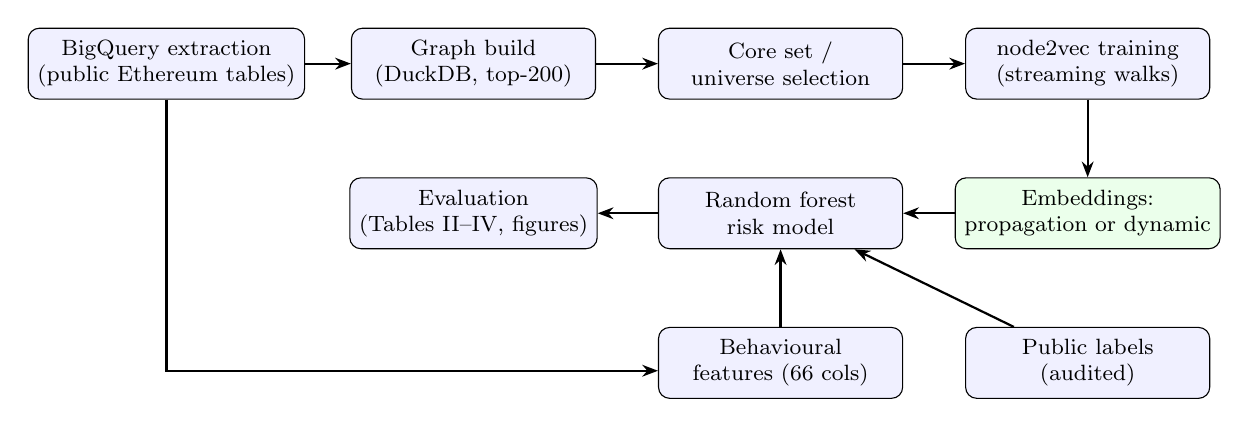
\begin{tikzpicture}[box/.style={draw,rounded corners,align=center,minimum height=9mm,minimum width=3.1cm,font=\footnotesize,fill=blue!6},
  arr/.style={-{Stealth[length=2mm]},thick}]
\node[box] (bq) at (0,0) {BigQuery extraction\\(public Ethereum tables)};
\node[box] (gr) at (3.9,0) {Graph build\\(DuckDB, top-200)};
\node[box] (co) at (7.8,0) {Core set /\\universe selection};
\node[box] (tr) at (11.7,0) {node2vec training\\(streaming walks)};
\node[box,fill=green!8] (em) at (11.7,-1.9) {Embeddings:\\propagation or dynamic};
\node[box] (rf) at (7.8,-1.9) {Random forest\\risk model};
\node[box] (ev) at (3.9,-1.9) {Evaluation\\(Tables II--IV, figures)};
\node[box] (fe) at (7.8,-3.8) {Behavioural\\features (66 cols)};
\node[box] (lb) at (11.7,-3.8) {Public labels\\(audited)};
\draw[arr] (bq)--(gr); \draw[arr] (gr)--(co); \draw[arr] (co)--(tr); \draw[arr] (tr)--(em);
\draw[arr] (em)--(rf); \draw[arr] (rf)--(ev); \draw[arr] (fe)--(rf); \draw[arr] (lb)--(rf);
\draw[arr] (bq) |- ([yshift=-1mm]fe.west);
\end{tikzpicture}
\caption{Overview of the reproduction pipeline. Every stage reads and writes files, so any stage can be rerun alone.}
\end{figure}

\subsection{Data extraction}
We extracted ETH transactions and ERC-20 transfer events from the public \texttt{crypto\_ethereum} BigQuery dataset, aggregating server-side to one row per address pair (count, value, first and last block) and one row per address and direction for behavioural statistics. The source tables are partitioned by timestamp, not block number, so each query filters on both: the timestamp prunes partitions (saving cost) and the block number makes the cut exact. A dry run estimated 48.6\,GiB of scanning, which the real run matched; every query carried a hard billing cap equal to its dry-run size plus 5\%. After download we verified that the highest block received is exactly 5\,000\,000, confirming the timestamp cap did not truncate data. A fast gRPC download was blocked by the machine's application-control policy, so results were fetched over REST in parallel, resumable range reads.

\subsection{Graph construction}
The global graph is built in staged DuckDB queries that spill to disk. Addresses are mapped to dense integer ids through a sorted list; joins use 64-bit hashes of addresses, with a collision check (none found). Pair weights are ETH transaction counts plus ERC-20 transfer counts, summed over both directions; each node keeps its top 200 neighbours by weight, as in the paper. The result has \NumNodes{} nodes. Random walks run over the undirected view (decision D13), because directed walks stall at sink addresses such as scam collectors.

\subsection{Behavioural features}
The paper's feature list (``Table~1'') is never given, so we defined \NumFeat{} features: for ETH (\NumFeatEth{} columns) and ERC-20 (\NumFeatErc{} columns) separately and for incoming and outgoing transfers, statistics of amount (count, sum, mean, standard deviation, min, max, median), counterparties, active days, timing (mean and standard deviation of gaps, span, burstiness) and in/out ratios. Heavy-tailed amounts are log-compressed before the forest, which leaves a tree model's information unchanged but avoids float32 overflow (D21).

\subsection{node2vec at laptop scale}
Walks are second-order biased walks implemented in Numba, with pre-drawn random numbers so results are deterministic regardless of thread scheduling. Because materialising all walks is impossible at millions of nodes, training streams walks in chunks to the skip-gram model; the vocabulary is built from expected visit frequencies (proportional to weighted degree) instead of a counting pass. We use dimension 128, window 10, 5 negatives, one epoch (all unspecified in the paper).

\subsection{Propagation, dynamic node2vec and the distributed walk generator}
\textbf{Core and propagation.} The core grows outward from the labeled addresses hop by hop up to 2.5\,M nodes, so that its induced subgraph is connected; a purely random 10\% sample would leave most nodes isolated. Embeddings of other addresses are the mean of up to five sampled one-hop core neighbours. We run two variants because the paper's core recipe is ambiguous: \emph{variant A}, where labeled addresses are core members and get trained embeddings, and \emph{variant B}, where they are kept out of the core and receive only propagated embeddings (decision D20).

\textbf{Dynamic node2vec.} The model is trained on the first snapshot; each update takes the addresses whose adjacency changed (delta nodes), generates walks from them over the full current graph, adds new addresses to the vocabulary and continues skip-gram training from the previous weights. Untouched addresses keep identical vectors, which we test.

\textbf{Distributed walks.} The split--apply--combine generator reads a neighbour store partitioned by source node, loading only the partitions it needs. By drawing its random numbers from the same stream as the in-memory generator it produces \emph{bit-identical} walks (tested, including across processes); we did not run it on a cluster.

\subsection{Risk model and evaluation protocol}
A random forest (500 trees, balanced class weights) is trained on an 80/20 split stratified by label and repeated over 5 seeds; we report mean and 95\% confidence interval. Splits are identical across all experiments, so comparisons are paired. Metrics are precision, recall and F$_1$ at threshold 0.5, PR-AUC and ROC-AUC. For Tables~III--IV the forest sees node2vec features only.

\subsection{Verification and bugs found along the way}
The code base (about 1\,800 lines in 18 modules, plus 16 scripts) has 61 automated tests, all passing at the time of writing. Testing and inspection found four defects worth recording because they could silently corrupt results elsewhere:
\begin{enumerate}
\item \textbf{Graph builder out of memory} on the first attempt at scale; rewritten as a staged, hash-keyed build verified equal to the in-memory builder.
\item \textbf{float32 overflow} from raw ERC-20 token units and in/out ratios (values above $10^{38}$); fixed by monotone log compression.
\item \textbf{gensim integer-token trap.} With integer tokens, gensim treats \texttt{n in model.wv} as true whenever $0\le n<|V|$ (it reads $n$ as a row index), so an incremental vocabulary update silently skips new nodes whose id is smaller than the vocabulary size. We reproduced this in isolation, switched all tokens to strings, and added a regression test that fails with integer tokens. This affects any dynamic-node2vec implementation that uses integer node ids with gensim.
\item \textbf{Leaky coverage flag.} A ``has embedding'' indicator correlated with the label (Section~\ref{sec:t2}); we quantified and controlled for it.
\end{enumerate}

%==================================================================================================
\section{Results: paper versus reproduction}
\label{sec:results}
\subsection{Table II: behavioural features, node2vec, and both}
\label{sec:t2}
Table~\ref{tab:t2} puts the paper's Table~II next to our two variants (all \NumLabeled{} labeled addresses). Table~\ref{tab:t2d} adds confidence intervals and control experiments.
\begin{table}[H]
\centering\footnotesize
\begin{tabular}{l ccc ccc ccc}
\toprule
 & \multicolumn{3}{c}{Paper} & \multicolumn{3}{c}{Ours, variant A} & \multicolumn{3}{c}{Ours, variant B}\\
\cmidrule(lr){2-4}\cmidrule(lr){5-7}\cmidrule(lr){8-10}
Features & P & R & F$_1$ & P & R & F$_1$ & P & R & F$_1$\\
\midrule
Behavioral features & 0.803 & 0.650 & 0.718 & 0.949 & 0.963 & 0.956 & 0.949 & 0.963 & 0.956\\
Node2vec embedding & 0.798 & 0.686 & 0.738 & 0.907 & 0.840 & 0.871 & 0.790 & 0.721 & 0.753\\
Node2vec + behavioral & 0.908 & 0.801 & 0.851 & 0.973 & 0.956 & 0.964 & 0.970 & 0.950 & 0.960\\
\bottomrule
\end{tabular}
\caption{Precision (P), recall (R) and F$_1$ at threshold 0.5. Paper values are from its Table~II. Variant A: labeled addresses are in the core; variant B: labeled addresses receive propagated embeddings only.}
\label{tab:t2}
\end{table}
\begin{table}[H]
\centering\scriptsize
\setlength{\tabcolsep}{3pt}\begin{tabular}{l r r ccc ccc}
\toprule
 & & & \multicolumn{3}{c}{F$_1$} & \multicolumn{3}{c}{PR-AUC}\\
\cmidrule(lr){4-6}\cmidrule(lr){7-9}
Variant & bad & good & behav. & n2v & both & behav. & n2v & both\\
\midrule
A: labeled in core & 481 & 4,080 & 0.956{\scriptsize$\pm$0.012} & 0.871{\scriptsize$\pm$0.018} & 0.964{\scriptsize$\pm$0.008} & 0.985{\scriptsize$\pm$0.009} & 0.939{\scriptsize$\pm$0.011} & 0.991{\scriptsize$\pm$0.006}\\
A, no miners & 481 & 127 & 0.982{\scriptsize$\pm$0.015} & 0.988{\scriptsize$\pm$0.004} & 0.987{\scriptsize$\pm$0.009} & 0.992{\scriptsize$\pm$0.012} & 0.992{\scriptsize$\pm$0.014} & 0.992{\scriptsize$\pm$0.013}\\
B: propagated & 481 & 4,080 & 0.956{\scriptsize$\pm$0.012} & 0.753{\scriptsize$\pm$0.029} & 0.960{\scriptsize$\pm$0.006} & 0.985{\scriptsize$\pm$0.009} & 0.829{\scriptsize$\pm$0.040} & 0.990{\scriptsize$\pm$0.005}\\
B, flag removed & 481 & 4,080 & 0.956{\scriptsize$\pm$0.012} & 0.746{\scriptsize$\pm$0.026} & 0.956{\scriptsize$\pm$0.009} & 0.985{\scriptsize$\pm$0.009} & 0.831{\scriptsize$\pm$0.041} & 0.990{\scriptsize$\pm$0.006}\\
B, covered only & 468 & 3,600 & 0.952{\scriptsize$\pm$0.016} & 0.760{\scriptsize$\pm$0.017} & 0.942{\scriptsize$\pm$0.011} & 0.985{\scriptsize$\pm$0.011} & 0.845{\scriptsize$\pm$0.025} & 0.986{\scriptsize$\pm$0.008}\\
B, no miners & 481 & 127 & 0.982{\scriptsize$\pm$0.015} & 0.932{\scriptsize$\pm$0.010} & 0.985{\scriptsize$\pm$0.013} & 0.992{\scriptsize$\pm$0.012} & 0.963{\scriptsize$\pm$0.014} & 0.992{\scriptsize$\pm$0.012}\\
\bottomrule
\end{tabular}
\caption{F$_1$ and PR-AUC with 95\% confidence intervals over 5 splits. ``Flag removed'' drops the has-embedding indicator; ``covered only'' keeps only addresses that have an embedding; ``no miners'' drops miners from the good class (481 bad, 127 good).}
\label{tab:t2d}
\end{table}
\textbf{Observations.}
\begin{itemize}
\item \emph{Absolute level.} Our behavioural F$_1$ (0.956) is far above the paper's (0.718), consistent with the easy, miner-dominated negative class (Section~\ref{sec:constraints}). Without miners, variant A saturates (all three feature sets 0.98--0.99, indistinguishable); in variant B node2vec alone reaches 0.932 and the other two 0.98.
\item \emph{Graph versus behavioural.} In the paper node2vec beats behavioural features, narrowly (0.738 against 0.718; no uncertainty given). On our data the order reverses: node2vec scores 0.871 (variant A) and 0.753 (variant B) against 0.956 for behaviour.
\item \emph{The combination.} The paper reports a large complementary gain (0.851, +0.113 over its best single set). Ours is +0.008 for variant A and +0.004 for variant B, inside the confidence intervals; on the clean covered-only subset the combination (0.942) is nominally \emph{below} behaviour alone (0.952). A ceiling effect is the likely reason: behaviour already scores 0.956, leaving little to gain.
\item \emph{Propagation costs accuracy.} Moving from trained embeddings (A, 0.871) to propagated ones (B, 0.753) lowers node2vec-only F$_1$ by 0.12, the pattern the paper uses to motivate the dynamic method.
\item \emph{A leak, found and controlled.} In variant B, 97.3\% of bad but only 88.2\% of good addresses received an embedding, so a has-embedding flag leaks the label. Of the 493 uncovered labeled addresses, 480 are miners, and 73\% of them touch only other labeled addresses (which variant B bars from the core). Removing the flag changed node2vec-only F$_1$ from 0.753 to 0.746; evaluating only covered addresses gives 0.760. The conclusion is unaffected, but the paper's setup could contain a similar coverage effect that is not discussed.
\end{itemize}

\subsection{Feature importance}
The paper states that the node2vec feature has very high importance. Table~\ref{tab:imp} shows grouped random-forest importance in our models. Node2vec carries 56.3\% (A) and 46.7\% (B) of total importance, consistent with the claim, but the group has 129 columns against 66 behavioural ones and impurity importance is biased towards groups with more columns, so this agrees with the claim only weakly. The behavioural ERC-20 group matters little (about 6\%), plausibly because few labeled addresses were active in ERC-20 transfers by 2018.
\begin{table}[H]
\centering\footnotesize
\begin{tabular}{l r r r}
\toprule
Feature group & columns & variant A & variant B\\
\midrule
Behavioral, ETH & 32 & 37.7\% & 47.4\%\\
Behavioral, ERC-20 & 34 & 6.0\% & 5.9\%\\
Node2vec (128 dims + flag) & 129 & 56.3\% & 46.7\%\\
\bottomrule
\end{tabular}
\caption{Grouped random-forest importance (combined feature set).}
\label{tab:imp}
\end{table}

\subsection{Coverage of propagation}
\begin{table}[H]
\centering\footnotesize
\begin{tabular}{p{7.6cm} r p{5.2cm}}
\toprule
Setting & Coverage & Detail\\
\midrule
Paper: propagation, whole Ethereum graph & 78\% & (80--85\% of daily-active addresses)\\
Ours, variant A: core 2.5M (labeled in core), whole 24.1M-node graph & 74.5\% & 17,943,148 of 24,084,076 nodes with an edge\\
Ours, variant B: labeled addresses kept out of the core, whole graph & 57.7\% & 13,894,934 of 24,084,076\\
Ours, variant B: labeled addresses embedded by propagation & 89.2\% & 97.3\% of bad, 88.2\% of good\\
Ours, Table IV universe (3M nodes), block 4.0M: core reach / labeled embedded & 97.9\% & 2,690 of 3,412 labeled\\
Ours, Table IV universe (3M nodes), block 4.5M: core reach / labeled embedded & 99.3\% & 3,735 of 4,225 labeled\\
Ours, Table IV universe (3M nodes), block 5.0M: core reach / labeled embedded & 100.0\% & 4,068 of 4,561 labeled\\
\bottomrule
\end{tabular}
\caption{Share of addresses that propagation can embed (core members plus addresses with at least one core neighbour).}
\label{tab:cov}
\end{table}
Coverage is highly setup-dependent. On the whole graph, variant A reaches \CovA\% (paper: 78\%) but variant B only \CovB\%, because excluding the labeled seeds changes which neighbourhoods fill the core. Inside our 3\,M-node universe, which is a ball around the labeled addresses, the core reaches 98--100\% of nodes, yet propagation still misses 11--21\% of the labeled addresses themselves. We therefore regard the paper's 78\% as neither confirmed nor contradicted.

\subsection{Table III: node2vec hyperparameter sweep}
We trained all 15 unique configurations of the paper's grid on the same core and scored each by the PR-AUC of a forest on node2vec features alone. The paper's differences between neighbouring settings are small (for example 0.751 versus 0.753), so we also retrained the base configuration ($3$ walks, length 8) with \NoiseN{} different seeds to measure noise. Its PR-AUC ranged from \NoiseLo{} to \NoiseHi{} (standard deviation \NoiseStd{}, range \NoiseRange{}). Table~\ref{tab:sweep} marks each result as above, below or within this band.
\begin{table}[H]
\centering\scriptsize
\begin{tabular}{rrrr cc c c r l}
\toprule
walks & len. & $p$ & $q$ & PR-AUC (all) & F$_1$ & PR-AUC (no miners) & paper AUC & train s & vs.\ noise\\
\midrule
3 & 4 & 1 & 1 & 0.693{\scriptsize$\pm$0.019} & 0.598 & 0.988 & (blank) & 97 & below\\
3 & 8 & 0.25 & 1 & 0.821{\scriptsize$\pm$0.016} & 0.732 & 0.996 & (blank) & 175 & below\\
3 & 8 & 0.5 & 1 & 0.846{\scriptsize$\pm$0.019} & 0.748 & 0.994 & 0.759 & 176 & within\\
3 & 8 & 1 & 0.25 & 0.870{\scriptsize$\pm$0.008} & 0.805 & 0.995 & (blank) & 174 & above\\
3 & 8 & 1 & 0.5 & 0.847{\scriptsize$\pm$0.019} & 0.745 & 0.993 & 0.753 & 180 & within\\
3 & 8 & 1 & 1 & 0.865{\scriptsize$\pm$0.014} & 0.782 & 0.994 & 0.751 & 169 & base\\
3 & 8 & 1 & 2 & 0.850{\scriptsize$\pm$0.006} & 0.746 & 0.995 & 0.767 & 174 & within\\
3 & 8 & 1 & 4 & 0.857{\scriptsize$\pm$0.012} & 0.770 & 0.995 & 0.767 & 170 & within\\
3 & 8 & 2 & 1 & 0.855{\scriptsize$\pm$0.018} & 0.782 & 0.992 & 0.753 & 175 & within\\
3 & 8 & 4 & 1 & 0.861{\scriptsize$\pm$0.021} & 0.768 & 0.993 & 0.767 & 175 & within\\
3 & 16 & 1 & 1 & 0.871{\scriptsize$\pm$0.014} & 0.781 & 0.993 & 0.774 & 375 & above\\
6 & 8 & 1 & 1 & 0.915{\scriptsize$\pm$0.006} & 0.841 & 0.994 & 0.787 & 317 & above\\
9 & 8 & 1 & 1 & 0.929{\scriptsize$\pm$0.008} & 0.863 & 0.993 & 0.795 & 461 & above\\
10 & 10 & 1 & 1 & 0.947{\scriptsize$\pm$0.008} & 0.893 & 0.992 & 0.814 & 675 & above\\
9 & 16 & 1 & 1 & 0.938{\scriptsize$\pm$0.013} & 0.852 & 0.991 & 0.808 & 1105 & above\\
\bottomrule
\end{tabular}
\caption{Sweep results (PR-AUC = area under the precision--recall curve; paper column is its undefined ``AUC'', so compare orderings, not values). ``vs.\ noise'' compares with the \NoiseLo--\NoiseHi{} band of retraining noise. Train s = seconds to train.}
\label{tab:sweep}
\end{table}
\textbf{Observations.}
\begin{itemize}
\item \emph{More walks help} (3 $\to$ 6 $\to$ 9: 0.865, 0.915, 0.929), as in the paper (0.751, 0.787, 0.795). Both settings lie above the noise band relative to the base, but the step from 6 to 9 walks (+0.014) is smaller than the noise range, so only the first step is clear.
\item \emph{Very short walks hurt} (length 4: 0.693). The paper's length-4 cell is blank.
\item \emph{Length 8 versus 16} is a marginal difference: 0.871 sits only 0.006 above the top of the noise band (0.841--0.865), far less than the band's 0.024 range, so we do not call it a gain, whereas the paper reports a small one (0.751 to 0.774).
\item \emph{Return and in-out parameters.} The paper finds $p=4$ and $q=2,4$ marginally better than 1. All our $p$ and $q$ settings lie between 0.821 and 0.870, a spread comparable to the noise range. The table flags $p=0.25$ (0.821, below the band) and $q=0.25$ (0.870, above it by only 0.005), but we do not regard either as a finding, so the paper's small $p,q$ effects are not distinguishable from noise on our data.
\item \emph{Best overall:} \BestWalks{} walks of length \BestLen{} with $p=q=1$ (PR-AUC \BestPRAUC), the paper's own choice. The (9,16) setting (0.938) is statistically indistinguishable and 64\% slower to train.
\item \emph{Consistency check.} The (10,10) result (\TenTenPRAUC) matches the independent Table~II node2vec-only run (\TableTwoNtvPRAUC) to within noise.
\end{itemize}
Precision--recall curves for the five parameter groups (the paper's Figures~5--9, labelled by the parameter actually varied) are in Appendix~\ref{app:figs}.

\subsection{Table IV: propagation versus dynamic node2vec}
The paper compares both methods at checkpoints and reports (AUC; propagation / dynamic): $(3,8)$ at 10\,M blocks 0.649/0.782; $(3,8)$ at 16\,M 0.686/0.860; $(10,10)$ at 10\,M 0.684/0.875, a gap of 0.13--0.19. We run both methods at 4.0\,M, 4.5\,M and 5.0\,M blocks with the (10,10) configuration, scoring them on the same labeled addresses (those present and embedded by both).
\begin{table}[H]
\centering\scriptsize
\begin{tabular}{r rrr rr cc cc}
\toprule
block & present & prop. & dyn. & bad & good & \multicolumn{2}{c}{PR-AUC} & \multicolumn{2}{c}{F$_1$}\\
\cmidrule(lr){7-8}\cmidrule(lr){9-10}
 & & embedded & embedded & \multicolumn{2}{c}{(shared set)} & prop. & dyn. & prop. & dyn.\\
\midrule
4.0M & 3,412 & 2,690 & 3,412 & 34 & 2,656 & 0.395{\scriptsize$\pm$0.107} & 0.498{\scriptsize$\pm$0.144} & 0.345 & 0.334\\
4.5M & 4,225 & 3,735 & 4,225 & 257 & 3,478 & 0.809{\scriptsize$\pm$0.037} & 0.846{\scriptsize$\pm$0.051} & 0.705 & 0.717\\
5.0M & 4,561 & 4,068 & 4,561 & 468 & 3,600 & 0.837{\scriptsize$\pm$0.026} & 0.922{\scriptsize$\pm$0.012} & 0.758 & 0.849\\
\bottomrule
\end{tabular}
\caption{Propagation versus dynamic node2vec, node2vec features only. ``Shared set'' = labeled addresses present at that block and embedded by both methods; PR-AUC and F$_1$ are scored there.}
\label{tab:t4}
\end{table}
\textbf{Observations.}
\begin{itemize}
\item \emph{Direction reproduces} at all three checkpoints (PR-AUC gaps +0.103, +0.037, +0.085), but intervals overlap at 4.0\,M (34 bad addresses only) and 4.5\,M. At 5.0\,M the gap is clear: \TFourDynPR{} versus \TFourPropPR{} PR-AUC, and F$_1$ 0.849 versus 0.758.
\item \emph{Coverage advantage.} Dynamic node2vec embedded every present labeled address at every checkpoint; propagation missed 21\%, 12\% and 11\%. Scored on all present addresses, dynamic reaches \DynAllPR{} PR-AUC at 5.0\,M.
\item \emph{Both improve over time,} as in the paper, but part of this is confounded with the growing number of bad addresses and more training data.
\item \emph{Cost.} The dynamic run took \DynSeconds{} s for all three checkpoints (it embeds the whole 3\,M-node universe); the propagation runs took \PropSeconds{} s in total (they embed a 1\,M-node core each time). At our scale the incremental method is therefore not faster; the paper's scalability argument concerns a graph two orders of magnitude larger, which we could not test.
\end{itemize}

\subsection{Figures 11--13: t-SNE of the embeddings}
\begin{figure}[H]
\centering
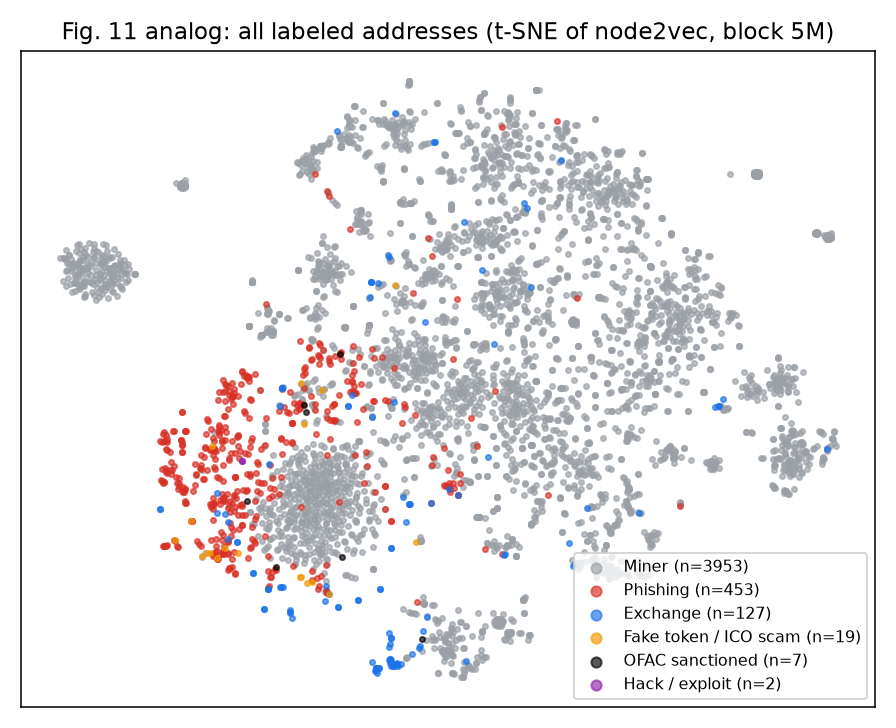
\includegraphics[width=0.62\textwidth]{figures/tsne_all}
\caption{Analog of the paper's Figure~11: t-SNE of dynamic node2vec embeddings (block 5\,M) for all labeled addresses. Phishing addresses (red) occupy a distinct region; miners (grey) cover most of the rest; exchanges (blue) are scattered.}
\end{figure}
\begin{figure}[H]
\centering
\begin{subfigure}{0.48\textwidth}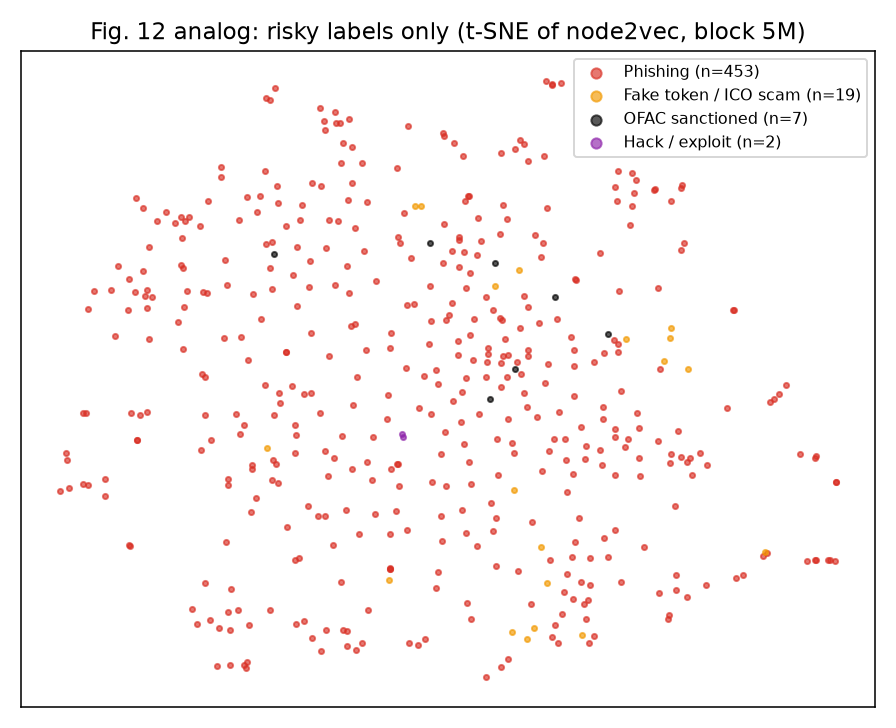
\includegraphics[width=\textwidth]{figures/tsne_risky}\caption{Risky labels only.}\end{subfigure}\hfill
\begin{subfigure}{0.48\textwidth}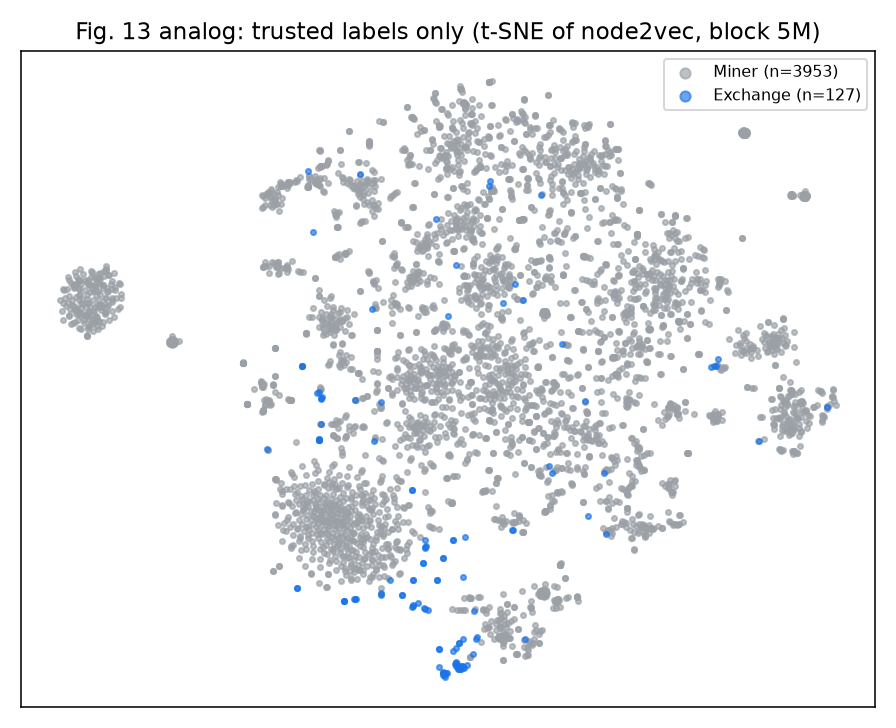
\includegraphics[width=\textwidth]{figures/tsne_trusted}\caption{Trusted labels only.}\end{subfigure}
\caption{Analogs of the paper's Figures~12 and~13, each projected separately.}
\end{figure}
``Visible clusters'' is a subjective criterion, so Table~\ref{tab:tsne} adds objective measures computed in the original 128-dimensional space, each next to a control with shuffled labels.
\begin{table}[H]
\centering\footnotesize
\begin{tabular}{l r cc cc c}
\toprule
 & $n$ & \multicolumn{2}{c}{silhouette (cosine)} & \multicolumn{2}{c}{5-NN accuracy} & majority\\
\cmidrule(lr){3-4}\cmidrule(lr){5-6}
 & & real & shuffled & real & shuffled & baseline\\
\midrule
Bad vs.\ good (all labeled) & 4,561 & 0.242 & -0.001 & 0.953 & 0.887 & 0.895\\
Six groups (Fig.~11 analog) & 4,559 & 0.011 & -0.070 & 0.938 & 0.857 & 0.867\\
Risky sub-types only (Fig.~12) & 479 & -0.148 & -0.068 & 0.948 & 0.946 & 0.942\\
Miners vs.\ exchanges (Fig.~13) & 4,080 & 0.457 & -0.014 & 0.979 & 0.969 & 0.969\\
\bottomrule
\end{tabular}
\caption{Cluster separation of the embeddings. Silhouette near 0 means no structure; 5-NN accuracy is 5-fold cross-validated and should be compared with the majority-class baseline.}
\label{tab:tsne}
\end{table}
The embedding separates the risk classes: bad versus good has a 5-NN accuracy of \TsneBadGoodKnn{} (balanced accuracy \TsneBadGoodBal) against a majority baseline of 0.895, and a silhouette of \TsneBadGoodSil{} (shuffled labels: $\approx$0). Miners and exchanges also separate (silhouette 0.457). Finer sub-types of risky addresses (fake-token scams, hacks, OFAC) do not separate beyond the baseline, but these classes are tiny (19, 2 and 7 addresses) and noisily tagged, so no conclusion is possible for them.

%==================================================================================================
\section{Analysis}
\label{sec:analysis}
\subsection{Claim-by-claim scorecard}
\label{sec:scorecard}
\begin{table}[H]
\centering\footnotesize
\begin{tabular}{p{3.9cm} p{3.2cm} p{4.7cm} p{2.5cm}}
\toprule
\textbf{Paper's claim} & \textbf{Paper} & \textbf{Our evidence} & \textbf{Verdict}\\
\midrule
Combining graph and behavioural features beats either alone (Table~II) & F$_1$ 0.851 vs.\ 0.738 / 0.718 & Gain +0.008 (A) / +0.004 (B), within noise; clean covered-only subset: 0.942 vs.\ 0.952 behaviour alone & \vNo\\
Graph features beat behavioural features alone & 0.738 vs.\ 0.718 (gap 0.02, no CI) & Reversed: 0.871 (A), 0.753 (B) vs.\ 0.956 & \vNo\\
Dynamic node2vec beats propagation (Table~IV) & Gap 0.13--0.19 AUC at all checkpoints & Higher at all three checkpoints (+0.103, +0.037, +0.085 PR-AUC); clear only at 5.0\,M; full coverage vs.\ 79--89\% & \vPart\\
Best setting is 10 walks, length 10, $p=q=1$; more walks help (Table~III) & Best 0.814; walks 0.751 $\to$ 0.795 & Best \BestPRAUC{}; walks 0.865 $\to$ 0.929; $p,q$ effects within noise & \vOK\\
Propagation reaches about 78\% of addresses & 78\% (80--85\% of daily-active) & \CovA\% (A) and \CovB\% (B) on the whole graph; 98--100\% in our universe & \vPart\\
Embeddings show label clusters (Figs.\ 11--13) & Qualitative & Bad vs.\ good separable (5-NN \TsneBadGoodKnn{} vs.\ 0.895 baseline); sub-types not separable (tiny classes) & \vPart\\
Node2vec has high feature importance & Stated, not shown & 56.3\% (A), 46.7\% (B), biased by column count & \vPart\\
Scales to every address and updates incrementally & Deployed at 266\,M & Demonstrated on a 3\,M-node universe (checkpoint updates, bit-identical distributed walks); not tested at paper scale & untestable here\\
\bottomrule
\end{tabular}
\caption{Scorecard. ``Reproduced'' means the ordering or trend holds on our data, not that absolute numbers match.}
\end{table}

\subsection{Why do the headline claims differ?}
We rank explanations by how well our evidence supports them.
\begin{enumerate}
\item \textbf{Ceiling effect from an easy negative class (well supported).} Behavioural features alone reach F$_1$ 0.956, and with exchanges as the only negatives every feature set in variant A saturates at 0.98--0.99. When behaviour already separates the classes, there is little for graph embeddings to add. The paper's much lower behavioural score (0.718) leaves room for the complementary gain it reports.
\item \textbf{Different negative class (plausible).} Our negatives are miners and exchanges; the paper's include government addresses and, plausibly, a broader mix. We cannot verify this because its labels are private.
\item \textbf{Label noise and era mismatch (plausible, unmeasured).} Our labels are a 2022 snapshot of Etherscan tags applied to 2015--2018 activity, and labeled bad addresses may have been well known and structurally distinctive; the paper's labels come largely from curated internal sources plus undisclosed external ones.
\item \textbf{Scale (plausible).} Neighbourhood structure in a graph 11 times smaller and five years earlier may carry less signal. The coverage numbers show the geometry differs.
\item \textbf{Embedding quality at fixed budget (possible).} We trained one epoch at dimension 128 with unspecified skip-gram settings. Better-tuned embeddings could narrow the gap, but our sweep shows large gains from more walks, which suggests the node2vec features are not yet saturated; a longer training would be a cheap check.
\end{enumerate}

\subsection{What we can and cannot conclude}
We can conclude that the paper's \emph{engineering} claims hold up in direction: node2vec settings, the benefit of incremental embedding over propagation (with full coverage), and the practicality of a streaming, partitioned pipeline. We cannot confirm or refute its headline ablation, because our data differ in exactly the ways that would hide or reverse such an effect. We did \emph{not} find evidence that the paper is wrong; we found that the claim is fragile to the negative class.

\subsection{Threats to validity}
\begin{itemize}
\item \textbf{Single training run per method} in Tables~II and IV. The reported intervals reflect random train/test splits of fixed embeddings, not retraining variation, which we measured at about 0.01 PR-AUC (Section~\ref{sec:results}). Part of the Table~IV gap could be training noise.
\item \textbf{Small bad class}, 481 addresses in total and 34 at the first checkpoint, makes some rows noisy.
\item \textbf{No external test set or temporal split.} Train and test addresses come from the same pool, as in the paper; a time-ordered split would be stricter.
\item \textbf{Label provenance} (Etherscan-derived) carries selection bias and a terms-of-use caveat.
\item \textbf{Multiple comparisons.} We inspected many configurations; the noise band guards against over-reading, but isolated differences should not be treated as findings.
\item \textbf{Unweighted snapshots, a 3\,M-node universe and a core that is a third of it} in Table~IV differ from the paper's larger core share relative to its universe.
\end{itemize}

%==================================================================================================
\section{Inconsistencies and gaps found in the paper}
We list these neutrally; none changes our conclusions but each made reproduction harder.
\begin{enumerate}
\item The behavioural features are said to be ``defined in Table~1'', but Table~I is the data-source table; the feature list is never given.
\item The text says the hyperparameter AUC values are in ``Table~II''; they are in Table~III. Table~II is the feature-set comparison.
\item Table~III has blank cells (for example length~4, $p=0.25$ and $q=0.25$ rows).
\item The captions of Figures~8 and~9 appear swapped: Figure~8 is titled ``In-out Parameter (p)'' and Figure~9 ``Return parameter (q)''.
\item The graph size is given as about 266\,M addresses in the introduction and about 275\,M in the conclusion.
\item The dynamic-node2vec citation points to reference~[2], an unrelated paper on money laundering (dynnode2vec is reference~[11]), and the MapReduce citation points to reference~[3], also unrelated.
\item References [12] and [14] are the same paper listed with different years.
\item The hardware section mentions CPUs, PyTorch and ``GNN models'', although the system uses node2vec with gensim, and a footnote describes a V100 GPU.
\item The incremental step is described as ``daily'' while checkpoints are millions of blocks apart (about 830 daily steps from 10\,M to 16\,M); the actual step size is unclear.
\item The metric called ``AUC'' in Tables~III and~IV is not defined; Table~II's classification threshold is not stated; no uncertainty is reported anywhere.
\item Minor: the organisation paragraph refers to Section~6 for the conclusion (it is Section~V); ``Propogation'' is misspelled in an algorithm title.
\end{enumerate}

%==================================================================================================
\section{Conclusions and next steps}
We built the complete system the paper describes, scaled it down to one machine, verified the components with tests, and ran every experiment the public data allowed. The paper's hyperparameter conclusions reproduce, and its dynamic-embedding advantage reproduces in direction with a clear margin at the final checkpoint and a decisive advantage in coverage. Its headline ablation does not reproduce on our easy, miner-dominated labels, and we explain why that is expected from our constraints, and what would be needed to test it properly.

\paragraph{Recommended next steps.}
\begin{enumerate}
\item \textbf{A stricter benchmark:} use ordinary, unlabeled accounts as negatives, evaluate on a time-ordered split, and report with and without miners.
\item \textbf{More labels and a larger tier:} extend the extraction to blocks 10\,M or 16\,M, where far more phishing and sanctioned addresses exist.
\item \textbf{Retraining variation:} repeat every embedding with several seeds so that all comparisons carry training-noise intervals.
\item \textbf{Improvements the baseline now allows us to measure:} inductive graph neural networks (which embed unseen addresses natively), time- and amount-aware walks, gradient-boosted classifiers with calibrated scores, and explainability for the risk score.
\end{enumerate}

\appendix
\section{Decision log}
\label{app:decisions}
Every place where the paper was silent or ambiguous, and every deviation, was logged when it was made.
{\footnotesize
\begin{longtable}{p{0.7cm} p{2.1cm} p{3.2cm} p{4.2cm} p{3.6cm}}
\toprule
\# & Topic & Paper says & Our choice & Reason\\
\midrule
\endhead
D1 & Behavioral feature list & References "Table 1" for features, but Table I is the data-source table. Says features are based on timestamp, amount, frequency of in/out transactions, for ETH and ERC-20 separately & Own list: amount stats, time stats, frequency, counterparties, in/out ratios, per ETH and ERC-20 & Matches the paper's textual description\\[2pt]
D2 & Embedding dimension & Not stated & 128 & node2vec default\\[2pt]
D3 & Skip-gram window / negatives / epochs & Not stated & window 10, negative 5, epochs 1 & gensim-typical defaults\\[2pt]
D4 & Propagation aggregation & "Aggregated embeddings of 5 sampled one-hop core neighbours" & Mean & Simplest, order-invariant\\[2pt]
D5 & Random forest & Not stated beyond "random forest" & 500 trees, class\_weight balanced & Standard, robust to imbalance\\[2pt]
D6 & Train/test split & Not stated & 80/20 stratified by address, fixed seeds, 5 seeds & Standard\\[2pt]
D7 & Decision threshold for P/R/F1 & Not stated & 0.5, plus PR-AUC and ROC-AUC reported & Threshold-free metrics avoid dependence\\[2pt]
D8 & Incremental step size & "Daily" training, but 10M->16M blocks at daily steps is \textasciitilde{}830 runs & \texttt{dynamic.step\_\allowbreak{}blocks} config (default 100K blocks), ablated & Almost certainly coarser in practice\\[2pt]
D9 & Edge definition & Directed; transactions between addresses & Directed, weight = interaction count (ETH + ERC-20) & Top-K ranking uses interaction count\\[2pt]
D10 & Table III / Figs 8-9 inconsistencies & Blank cells; p/q captions appear swapped & Run the full grid ourselves, do not trust captions & Cross-check\\[2pt]
D11 & Labels & Private (Coinbase internal + undisclosed external) & Public sources (to be assembled in M3) & Biggest deviation; judged by claims, not absolute numbers\\[2pt]
D12 & Development data & n/a & Synthetic world with planted fraud clusters (M1) before real data & Fast, deterministic debugging; real-data results are what count for the reproduction\\[2pt]
D13 & Walk direction & "Directed edges correspond to transactions" & Walks run over the undirected view (neighbors = in + out); \texttt{directed=True} available in \texttt{build\_\allowbreak{}graph} & A pure out-edge walk gets stuck at sinks (fraud collectors, cold wallets); propagation also uses "directly transacted" in either direction\\[2pt]
D14 & Walk edge weights & Top-K neighbors are chosen by interaction count; walk bias not specified & Weighted walks (probability proportional to interaction count x p/q factor) & Reference node2vec semantics; ablatable via \texttt{weighted} flag\\[2pt]
D15 & Distributed walk fidelity & "MapReduce split-apply-combine" & Per-walk uniforms taken from the same PCG64 stream as the in-memory generator, so the partitioned output is bit-identical (tested) & Proves distribution changes nothing about the algorithm\\[2pt]
D16 & Propagation vs dynamic training graph & Both "at similar checkpoints" & Propagation: node2vec on the \emph{induced subgraph of the core set} then one-hop propagation over the full graph; Dynamic: all addresses, incremental & Matches the paper's description of each method\\[2pt]
D17 & ERC-20 amounts & Not specified & Raw token units (decimals differ per token), plus distinct-token count; ETH value in ETH & Normalising needs a decimals table; revisit if ERC-20 features look unstable\\[2pt]
D18 & Extraction method & Not specified & Server-side aggregation in BigQuery with partition-pruning on block\_timestamp plus an exact block\_number cut; internal traces excluded & Avoids moving billions of raw rows; matches "transactions" and "ERC-20 transactions"\\[2pt]
D19 & eth-labels as a label source & n/a & \texttt{phish-hack} (bad) and \texttt{exchange} (good) files from dawsbot/eth-labels (MIT repo) used for development & The repo's data is scraped from Etherscan, whose terms of use are unclear; flagged to the user, who approved the download. Re-check before publishing results or redistributing the data\\[2pt]
D20 & Are labeled addresses in the core set? & "included all the addresses ... which have transacted with any addresses in the training set" (ambiguous) & Both variants are run: A) labeled addresses are core members (embeddings trained directly); B) labeled addresses are excluded from the core and only get propagated embeddings. Variant B is the faithful test of propagation & Cheap to run both; they answer different questions and the comparison is informative\\[2pt]
D21 & Heavy-tailed behavioral amounts & Not discussed & Behavioral features go through a monotone \texttt{sign(x)*log1p(|x|)} before the classifier & ERC-20 amounts are raw token units and in/out value ratios reach >1e38, overflowing float32 in the random forest; trees depend only on value ordering, so no information is lost\\[2pt]
D22 & Snapshots for Table IV & Daily-updated graph; edge counts per time step not specified & Time-sliced snapshots from each pair's first block, unweighted (exact counts per checkpoint are not in the extracted tables); each node keeps its top-200 neighbors by total count, then edges are filtered by first block & Edge existence never looks ahead; only the choice of which neighbors to keep uses final counts\\[2pt]
D23 & Table IV setup & Checkpoints 5M, 8M, 10M, 16M blocks; 30M-address core of 266M & Universe of 3M nodes around the labeled addresses, propagation core of 1M (labeled excluded), checkpoints 4.0M, 4.5M, 5.0M with an update every 250K blocks, configuration (10,10,1,1) throughout & Bad labels are scarce before 4M blocks (36 present at 4.0M); a 3M universe fits in 15.7 GiB at dimension 128; the core must be large enough to contain the labeled addresses' neighbors\\[2pt]
D24 & Table III protocol & Sweep on a 30M-address subsample; metric called AUC & Sweep on the 2.5M-node core subgraph, node2vec-only random-forest PR-AUC (area under the precision-recall curve), identical splits for all runs, and 3 extra training seeds of the base configuration to measure retraining noise & Differences in the paper are as small as 0.002, so noise had to be measured; PR-AUC is the paper's stated evaluation metric family\\[2pt]
\bottomrule
\end{longtable}
}

\section{Reproducibility}
\label{app:repro}
\textbf{Environment.} Windows 11, 16 cores, 15.7\,GiB RAM, Python 3.12; main libraries: NumPy, pandas, DuckDB, scikit-learn, gensim 4.4, Numba, PyArrow. This report was typeset with Tectonic.

\textbf{Pipeline order} (all scripts in \texttt{scripts/}, tests in \texttt{tests/}):
\begin{enumerate}[label=\arabic*.]
\item \texttt{bq\_dry\_run.py}, \texttt{extract\_bq.py}: dry-run costs, then extract and download the BigQuery tables (parallel, resumable, billing-capped).
\item \texttt{label\_overlap.py}, \texttt{real\_features.py}: label audit and behavioural features for labeled addresses.
\item \texttt{train\_core.py}: core selection and node2vec training (\texttt{--exclude-seeds} for variant B); \texttt{table2\_real.py}: Table~II.
\item \texttt{build\_snapshots.py}, \texttt{table4\_run.py}, \texttt{table4\_eval.py}: time-sliced adjacency, propagation and dynamic runs, Table~IV.
\item \texttt{sweep\_table3.py}, \texttt{sweep\_report.py}: Table~III sweep and its figures.
\item \texttt{tsne\_figures.py}, \texttt{make\_report\_tables.py}: t-SNE figures and every table in this report, generated from result files.
\end{enumerate}
Raw data, graphs and embeddings are not under version control (large, regenerable, and some label sources have unclear terms of use).

\section{Additional figures}
\label{app:figs}
\begin{figure}[H]
\centering
\begin{subfigure}{0.48\textwidth}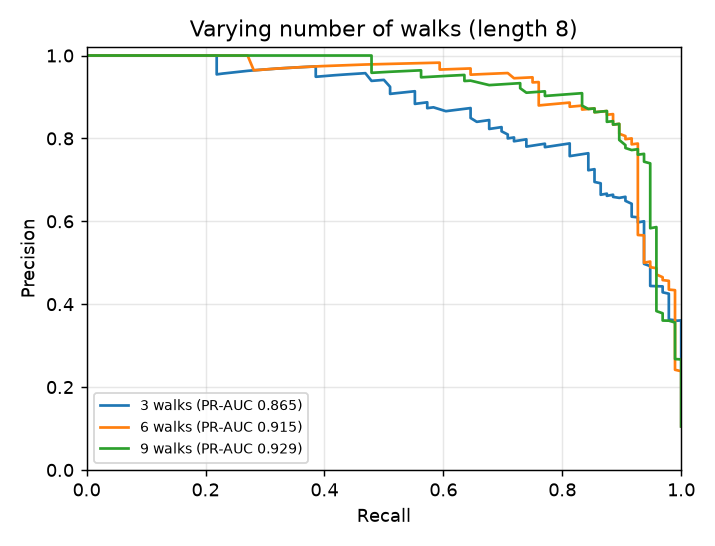
\includegraphics[width=\textwidth]{figures/sweep_fig5_walks}\end{subfigure}\hfill
\begin{subfigure}{0.48\textwidth}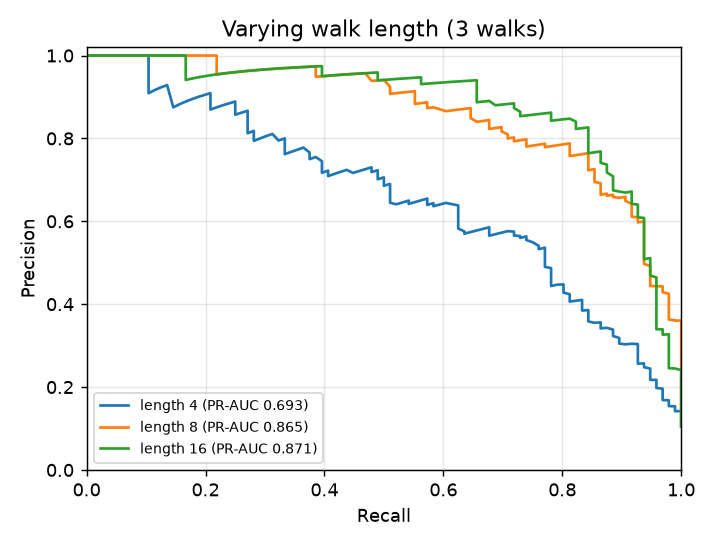
\includegraphics[width=\textwidth]{figures/sweep_fig6_length}\end{subfigure}\\[4pt]
\begin{subfigure}{0.48\textwidth}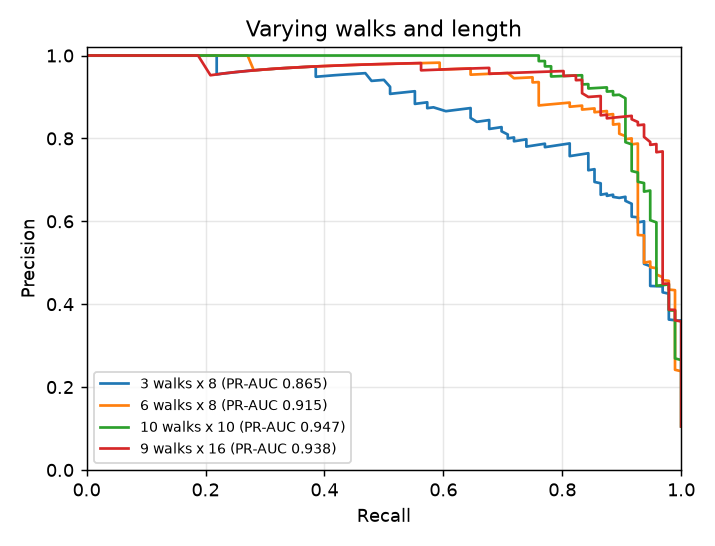
\includegraphics[width=\textwidth]{figures/sweep_fig7_joint}\end{subfigure}\hfill
\begin{subfigure}{0.48\textwidth}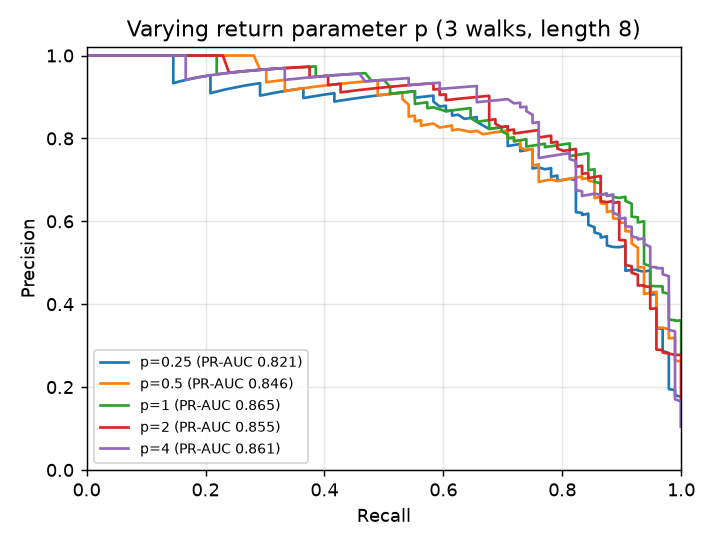
\includegraphics[width=\textwidth]{figures/sweep_fig8_p}\end{subfigure}\\[4pt]
\begin{subfigure}{0.48\textwidth}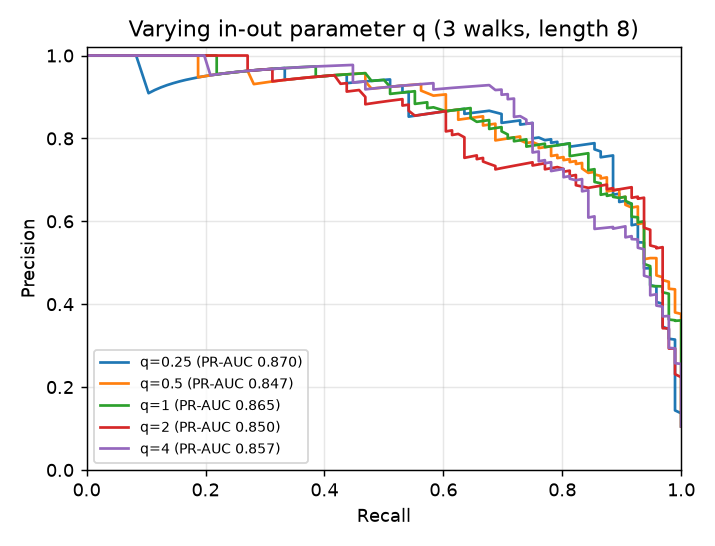
\includegraphics[width=\textwidth]{figures/sweep_fig9_q}\end{subfigure}
\caption{Precision--recall curves of the Table~III sweep (analogs of the paper's Figures~5--9; one curve per setting from the first test split, legends give the mean PR-AUC over five splits). Panels: walks, length, joint walks and length, return parameter $p$, in-out parameter $q$.}
\end{figure}

\end{document}
